\section{Incompressible Navier-Stokes Solver}

3.4/UserGuide/Tutorial/IncNavierStokesSolver
3.4/UserGuide/Tutorial/IncNavierStokesSolver/Stability
3.4/UserGuide/Examples/IncNavierStokesSolver/Adjoint
3.4/UserGuide/Examples/IncNavierStokesSolver/Aorta
3.4/UserGuide/Examples/IncNavierStokesSolver/Biglobal
3.4/UserGuide/Examples/IncNavierStokesSolver/Direct
3.4/UserGuide/Examples/IncNavierStokesSolver/KovasznayFlow2D
3.4/UserGuide/Examples/IncNavierStokesSolver/LaminarChannelFlow2D
3.4/UserGuide/Examples/IncNavierStokesSolver/LaminarChannelFlow2DLinNS

\newpage
3.4/UserGuide/Examples/IncNavierStokesSolver/LaminarChannelFlow3D
\subsection{Laminar Channel Flow 3D}
The following example demonstrates the application of the \textbf{IncNavierStokesSolver  (REF?)} using the \textbf{Velocity Correction Scheme (REF?)} algorithm for modelling 3D laminar channel flow.

\subsubsection{Background}
The governing equation is the unsteady incompressible Navier-Stokes equation:
\begin{equation}
\begin{cases}
\frac{\partial \textbf{u}}{\partial t} + \textbf{u} \cdot \nabla \textbf{u} = - \nabla p + \nu \nabla^2 \textbf{u} + f \\
\nabla \cdot \textbf{u} = 0
\end{cases}
\end{equation}

In the following we will numerically solve for the three dimensional velocity and pressure field for steady boundary conditions. The Reynolds number under consideration is 1.

\subsection{Geometry}
The geometry under consideration is a 3D square channel with unit length and height (\textit{i.e.} $D=1$). The channel is modelled using tetrahedral elements.

\subsection{Input parameters}
The session file can be found in the tests folder under the IncNavierStokesSolver folder and is named Tet\_channel\_m8\_par.xml.

\paragraph{Expansion:~} In this example we will use a 7th order polynomial expansion (\textit{i.e.} $P=8$).
\begin{lstlisting}[style=XMLStyle]
<EXPANSIONS>
  <E COMPOSITE="C[0]" NUMMODES="8" FIELDS="u,v,w,p" TYPE="MODIFIED" />
</EXPANSIONS>
\end{lstlisting}

\paragraph{Solver information:~} These information are given by
\begin{lstlisting}[style=XMLStyle]
<SOLVERINFO>
  <I PROPERTY="SolverType" VALUE="VelocityCorrectionScheme" />
  <I PROPERTY="EQTYPE" VALUE="UnsteadyNavierStokes" />
  <I PROPERTY="AdvectionForm" VALUE="Convective" />
  <I PROPERTY="Projection" VALUE="Galerkin" />
  <I PROPERTY="TimeIntegrationMethod" VALUE="IMEXOrder1" />
</SOLVERINFO>
\end{lstlisting}

\paragraph{Parameters:~} Setting the mean inlet velocity to 1, allows us to define the kinematic viscosity as $\nu = \frac{UD}{Re}=1$.
\begin{lstlisting}[style=XMLStyle]
<PARAMETERS>
  <P> TimeStep      = 0.001 </P>
  <P> NumSteps      = 10 </P>
  <P> IO_CheckSteps = 10    </P>
  <P> IO_InfoSteps  = 10    </P>
  <P> Kinvis        = 1   </P>
  <P> IterativeSolverTolerance = 1e-10 </P>
</PARAMETERS>
\end{lstlisting}

\paragraph{Boundary conditions:~} The boundary conditions are defined by
\begin{lstlisting}[style=XMLStyle]
        <BOUNDARYREGIONS>
            <B ID="0"> C[1] </B>    <!-- Inlet -->
            <B ID="1"> C[6] </B>    <!-- Outlet -->
            <B ID="2"> C[2] </B>    <!-- Wall -->
            <B ID="3"> C[3] </B>    <!-- Wall left -->
            <B ID="4"> C[4] </B>    <!-- Wall -->
            <B ID="5"> C[5] </B>    <!-- Wall right -->
        </BOUNDARYREGIONS>

        <BOUNDARYCONDITIONS>
            <REGION REF="0">
                <D VAR="u" VALUE="0" />
                <D VAR="v" VALUE="0" />
                <D VAR="w" VALUE="y*(1-y)" />
                <N VAR="p" USERDEFINEDTYPE="H" VALUE="0" />
            </REGION>
            <REGION REF="1">
                <N VAR="u" VALUE="0" />
                <N VAR="v" VALUE="0" />
                <N VAR="w" VALUE="0" />
                <D VAR="p" VALUE="0" />
            </REGION>
            <REGION REF="2">
                <D VAR="u" VALUE="0" />
                <D VAR="v" VALUE="0" />
                <D VAR="w" VALUE="0" />
                <N VAR="p" USERDEFINEDTYPE="H" VALUE="0" />
            </REGION>
            <REGION REF="3">
                <D VAR="u" VALUE="0" />
                <D VAR="v" VALUE="0" />
                <D VAR="w" VALUE="y*(1-y)" />
                <N VAR="p" USERDEFINEDTYPE="H" VALUE="0" />
            </REGION>
            <REGION REF="4">
                <D VAR="u" VALUE="0" />
                <D VAR="v" VALUE="0" />
                <D VAR="w" VALUE="0" />
                <N VAR="p" USERDEFINEDTYPE="H" VALUE="0" />
            </REGION>
            <REGION REF="5">
                <D VAR="u" VALUE="0" />
                <D VAR="v" VALUE="0" />
                <D VAR="w" VALUE="y*(1-y)" />
                <N VAR="p" USERDEFINEDTYPE="H" VALUE="0" />
            </REGION>
        </BOUNDARYCONDITIONS>
\end{lstlisting}

\paragraph{Functions:~} The exact solution is known in this case, and is therefore used to calculate the error.
\begin{lstlisting}[style=XMLStyle]
        <FUNCTION NAME="ExactSolution">
            <E VAR="u" VALUE="0" />
            <E VAR="v" VALUE="0" />
            <E VAR="w" VALUE="y*(1-y)" />
            <E VAR="p" VALUE="-2*Kinvis*(z-1)" />
        </FUNCTION>
        <FUNCTION NAME="InitialConditions">
            <E VAR="u" VALUE="0" />
            <E VAR="v" VALUE="0" />
            <E VAR="w" VALUE="y*(1-y)" />
            <E VAR="p" VALUE="-2*Kinvis*(z-1)" />
        </FUNCTION>
\end{lstlisting}

\subsubsection{Usage}
./IncNaverStokesSolver Tet\_channel\_m8\_par.xml

\subsubsection{Result}
\begin{figure}
\begin{center}
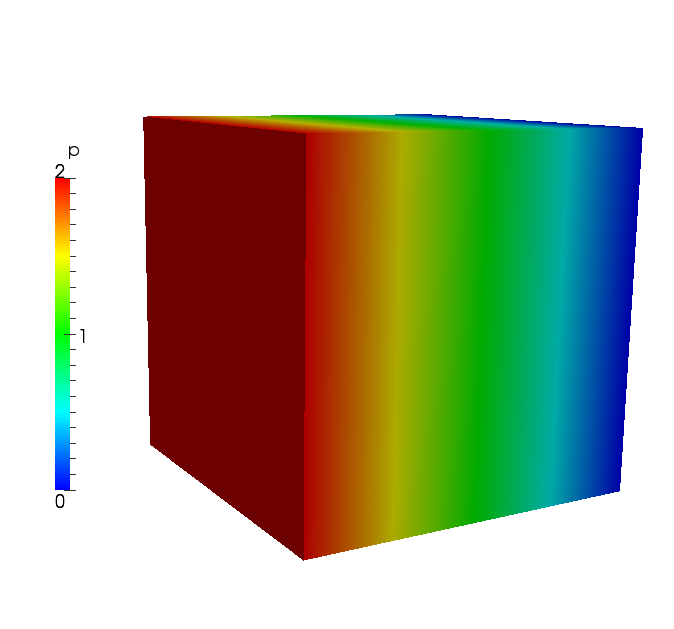
\includegraphics[width=7cm]{Figures/CF3DP8PR.png}
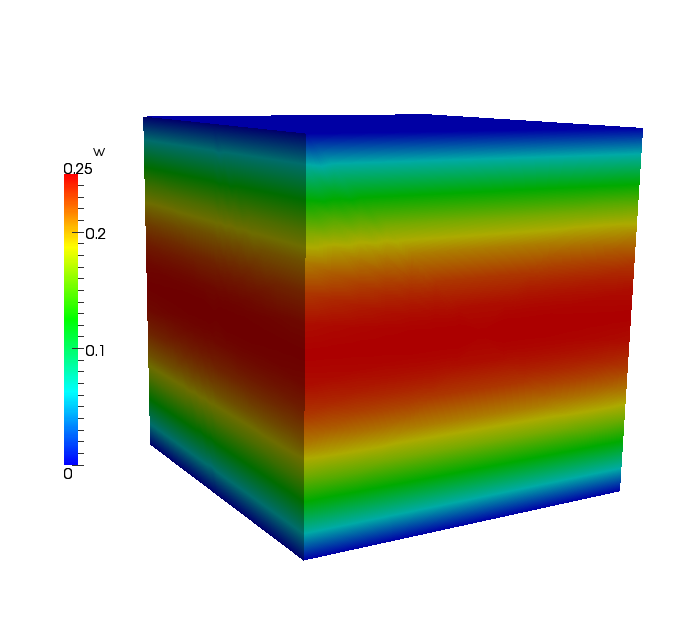
\includegraphics[width=7cm]{Figures/CF3DP8.png}
\caption{Pressure and velocity profiles for the laminar channel flow (full 3D).}
\end{center}
\end{figure}






\newpage
3.4/UserGuide/Examples/IncNavierStokesSolver/LaminarChannelFlow3DH1D
\subsection{Laminar Channel Flow Quasi-3D}
In this example we reuse the 2D mesh used before for the \textbf{2D Laminar Channel Flow (REF?)} example, and we add mathematically the third dimension assuming an expansion along z with a Fourier series. The example is an application of the \textbf{IncNavierStokesSolver  (REF?)} using the \textbf{Velocity Correction Scheme (REF?)} algorithm.

\subsubsection{Background}
The governing equation is the unsteady incompressible Navier-Stokes equation:
\begin{equation}
\begin{cases}
\frac{\partial \textbf{u}}{\partial t} + \textbf{u} \cdot \nabla \textbf{u} = - \nabla p + \nu \nabla^2 \textbf{u} + f \\
\nabla \cdot \textbf{u} = 0
\end{cases}
\end{equation}

The Reynolds number under consideration is 1.

\subsubsection{Geometry}
The geometry under consideration is a 2D square channel with unit length and height (\textit{i.e.} $D=1$). The channel is modelled using 4 quadrilateral elements. The geometry as well as the mesh is identical to that used in the \textbf{2D Laminar Channel Flow (REF?)} example.

\subsubsection{Input parameters}
\paragraph{Expansion:~} In this example we will use a quadratic polynomial expansion (\textit{i.e.} $P=3$).
\begin{lstlisting}[style=XMLStyle]
<EXPANSIONS>
  <E COMPOSITE="C[0]" NUMMODES="3" FIELDS="u,v,w,p" TYPE="MODIFIED" />
</EXPANSIONS>
\end{lstlisting}

\paragraph{Solver information:~}  The flag 
\begin{lstlisting}[style=XMLStyle] 
<I PROPERTY="HOMOGENEOUS" VALUE="1D"/> 
\end{lstlisting} 
is informing the code that, even if the mesh is 2D, the problem is 3D and the third direction needs to be added with a Fourier series. An extra flag could be added to activate the FFT routines inside the code 
\begin{lstlisting}[style=XMLStyle]
<I PROPERTY="USEFFT" VALUE="FFTW"/>
\end{lstlisting} 

In this case Nektar++ uses the FFTW library to move the degrees of freedom from wave to real space. HomModesZ and LZ set the number of Fourier modes and the length of the third direction respectively.
\begin{lstlisting}[style=XMLStyle]
  <SOLVERINFO>
    <I PROPERTY="EQTYPE" VALUE="UnsteadyNavierStokes"/>
    <I PROPERTY="SolverType"  VALUE="VelocityCorrectionScheme"/>
    <I PROPERTY="EvolutionOperator" VALUE="Nonlinear" />
    <I PROPERTY="Projection" VALUE="Galerkin"/>
    <I PROPERTY="TimeIntegrationMethod" VALUE="IMEXOrder3"/>
    <I PROPERTY="HOMOGENEOUS" VALUE="1D"/>
  </SOLVERINFO>
\end{lstlisting}

\paragraph{Parameters:~} Setting the mean inlet velocity to 1, allows us to define the kinematic viscosity as $\nu = \frac{UD}{Re}=1$.
\begin{lstlisting}[style=XMLStyle]
  <PARAMETERS>
    <P> TimeStep      = 0.001    </P>
    <P> NumSteps      = 1000     </P>
    <P> IO_CheckSteps = 1000     </P>
    <P> IO_InfoSteps  = 1000     </P>
    <P> Kinvis        = 1        </P>
    <P> HomModesZ     = 20       </P>
    <P> LZ            = 1.0      </P>
  </PARAMETERS>
\end{lstlisting}

\paragraph{Boundary conditions:~} Boundary conditions have been defined on the walls and at the inflow (regions 0 and 1) as Dirichlet for the velocity field and as high-order for the pressure. At the outflow the velocity is left free using Neumann boundary conditions and the pressure is set to zero using Dirichlet.
\begin{lstlisting}[style=XMLStyle]
  <BOUNDARYCONDITIONS>
    <REGION REF="0">
      <D VAR="u" VALUE="0" />
      <D VAR="v" VALUE="0" />
      <D VAR="w" VALUE="0" />
      <N VAR="p" USERDEFINEDTYPE="H" VALUE="0" />
    </REGION>
    <REGION REF="1">
      <D VAR="u" VALUE="y*(1-y)" />
      <D VAR="v" VALUE="0" />
      <D VAR="w" VALUE="0" />
      <N VAR="p" USERDEFINEDTYPE="H" VALUE="0" />
    </REGION>
    <REGION REF="2">
      <N VAR="u" VALUE="0" />
      <N VAR="v" VALUE="0" />
      <N VAR="w" VALUE="0" />
      <D VAR="p" VALUE="0" />
    </REGION>
  </BOUNDARYCONDITIONS>
\end{lstlisting}

\paragraph{Functions:~} Homogeneous initial conditions are imposed and an analytical formulation of the exact solution is provided.
\begin{lstlisting}[style=XMLStyle]
  <FUNCTION NAME="InitialConditions">
     <E VAR="u" VALUE="0" />
     <E VAR="v" VALUE="0" />
     <E VAR="w" VALUE="0" />
     <E VAR="p" VALUE="0" />
  </FUNCTION>

  <FUNCTION NAME="ExactSolution">
     <E VAR="u" VALUE="y*(1-y)" />
     <E VAR="v" VALUE="0" />
     <E VAR="w" VALUE="0" />
     <E VAR="p" VALUE="-2*Kinvis*(x-1)" />
  </FUNCTION>
\end{lstlisting}

\subsubsection{Usage}
./IncNaverStokesSolver session.xml

\subsubsection{Result}
\begin{figure}
\begin{center}
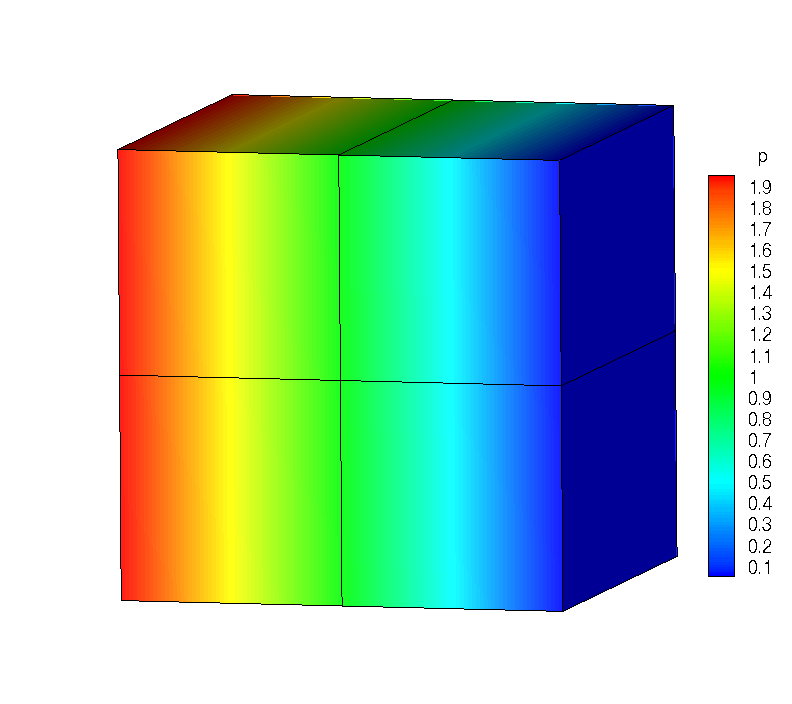
\includegraphics[width=7cm]{Figures/CF3DCVP3PR.png}
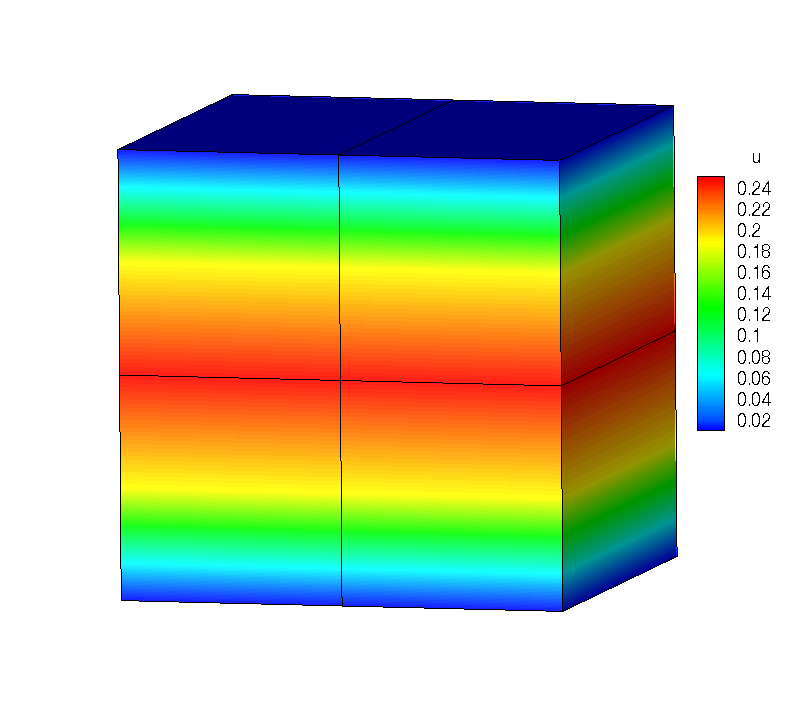
\includegraphics[width=7cm]{Figures/CF3DCVP3.png}
\caption{Pressure and velocity profiles for the laminar channel flow (quasi 3D).}
\end{center}
\end{figure}

\newpage









3.4/UserGuide/Examples/IncNavierStokesSolver/SteadyOseenFlow2D
3.4/UserGuide/Examples/IncNavierStokesSolver/Transient

\newpage
3.4/UserGuide/Examples/IncNavierStokesSolver/TurbulentChannelFlow
\subsection{Turbulent Channel Flow Quasi-3D}
In this example we use a 2D mesh for channel flow, and we add mathematically the third dimension assuming an expansion along z with a Fourier series. The example is an application of the \textbf{IncNavierStokesSolver  (REF?)} using the \textbf{Velocity Correction Scheme (REF?)} algorithm in order to solve for turbulent channel flow.

\subsubsection{Background}
The governing equation is the unsteady incompressible Navier-Stokes equation:
\begin{equation}
\begin{cases}
\frac{\partial \textbf{u}}{\partial t} + \textbf{u} \cdot \nabla \textbf{u} = - \nabla p + \nu \nabla^2 \textbf{u} + f \\
\nabla \cdot \textbf{u} = 0
\label{IncNS_equations}
\end{cases}
\end{equation}

The Reynolds number under consideration is 2000.

\subsubsection{Geometry}
The geometry under consideration is a 2D square channel with height of 2 units (\textit{i.e.} $D=2$), and length of 12.57. The channel is modelled using quadrilateral elements.
\begin{figure}
\begin{center}
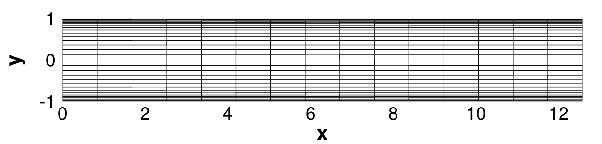
\includegraphics[width=10cm]{Figures/ChanMesh.png}
\caption{Mesh used for the turbulent channel flow (quasi-3D).}
\end{center}
\end{figure}

\subsubsection{Input parameters}
For this tutorial, the input file (in the \textbf{Nektar++ input format (REF?)}) used can be found in Nektar++/solvers/IncNavierStokesSolver/Examples/TurbChFl\_3DH1D.xml.

\paragraph{Expansion:~} In this example we will use a quadratic polynomial expansion (\textit{i.e.} $P=3$).
\begin{lstlisting}[style=XMLStyle]
<EXPANSIONS>
  <E COMPOSITE="C[0]" NUMMODES="3" FIELDS="u,v,w,p" TYPE="MODIFIED" />
</EXPANSIONS>
\end{lstlisting}

\paragraph{Solver information:~} The flag 
\begin{lstlisting}[style=XMLStyle]
<I PROPERTY="HOMOGENEOUS" VALUE="1D"/>
\end{lstlisting}
is informing the code that, even if the mesh is 2D, the problem is 3D and the third direction needs to be added with a Fourier series. An extra flag could be added to activate the FFT routines inside the code 
\begin{lstlisting}[style=XMLStyle]
<I PROPERTY="USEFFT" VALUE="FFTW"/>
\end{lstlisting}
In this case Nektar++ uses the FFTW library to move the degrees of freedom from wave to real space. HomModesZ and LZ set the number of Fourier modes and the length of the third direction respectively.

\begin{lstlisting}[style=XMLStyle]
    <SOLVERINFO>
      <I PROPERTY="SolverType"  VALUE="VelocityCorrectionScheme"/>
      <I PROPERTY="EQTYPE" VALUE="UnsteadyNavierStokes"/>
      <I PROPERTY="AdvectionForm" VALUE="Convective"/>
      <I PROPERTY="Projection" VALUE="Galerkin"/>
      <I PROPERTY="TimeIntegrationMethod" VALUE="IMEXOrder2"/>
      <I PROPERTY="HOMOGENEOUS" VALUE="1D"/>
    </SOLVERINFO>
\end{lstlisting}

\paragraph{Parameters:~} Setting the mean inlet velocity to 1, allows us to define the kinematic viscosity as $\nu = \frac{UD}{Re}=1$.
\begin{lstlisting}[style=XMLStyle]
    <PARAMETERS>
      <P> TimeStep      = 0.0001      </P>
      <P> NumSteps      = 10000       </P>
      <P> IO_CheckSteps = 1000       </P>
      <P> IO_InfoSteps  = 10       </P>
      <P> Re            = 2000       </P>
      <P> Kinvis        = 1.0/Re     </P>
      <P> HomModesZ     = 32          </P>
      <P> LZ            = 4*PI/3     </P>
    </PARAMETERS>
\end{lstlisting}

\paragraph{Boundary conditions:~} The boundary conditions are defined by
\begin{lstlisting}[style=XMLStyle]
    <BOUNDARYREGIONS>
      <B ID="0"> C[1] </B> //walls
      <B ID="1"> C[2] </B> //inflow
      <B ID="2"> C[3] </B> //outflow
    </BOUNDARYREGIONS>

    <BOUNDARYCONDITIONS>
      <REGION REF="0">
        <D VAR="u" VALUE="0" />
        <D VAR="v" VALUE="0" />
        <D VAR="w" VALUE="0" />
        <N VAR="p" USERDEFINEDTYPE="H" VALUE="0" />  
      </REGION>
      <REGION REF="1">
        <P VAR="u" VALUE="[2]" />
        <P VAR="v" VALUE="[2]" />
        <P VAR="w" VALUE="[2]" />
        <P VAR="p" VALUE="[2]" />
      </REGION>
      <REGION REF="2">
        <P VAR="u" VALUE="[1]" />
        <P VAR="v" VALUE="[1]" />
        <P VAR="w" VALUE="[1]" />
        <P VAR="p" VALUE="[1]" />
      </REGION>
    </BOUNDARYCONDITIONS>
\end{lstlisting}

\paragraph{Functions:~} The initial conditions and the body force (\textit{i.e.} $f$ in the governing equations \ref{IncNS_equations}) are given by
\begin{lstlisting}[style=XMLStyle]
   <FUNCTION NAME="InitialConditions">
     <E VAR="u" VALUE="1" />
     <E VAR="v" VALUE="0" />
     <E VAR="w" VALUE="0" />
     <E VAR="p" VALUE="0" />
   </FUNCTION>
   
   <FUNCTION NAME="BodyForce">
          <E VAR="u" VALUE="2*Kinvis" />
          <E VAR="v" VALUE="0" />
          <E VAR="w" VALUE="0" />
   </FUNCTION>
\end{lstlisting}

\subsubsection{Usage} ./IncNaverStokesSolver TurbChFl\_3DH1D.xml 

\subsubsection{Result}
\begin{figure}
\begin{center}
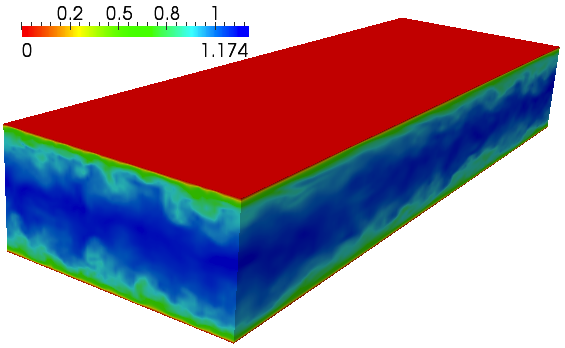
\includegraphics[width=12cm]{Figures/ChanCont.png}
\caption{Velocity profile of the turbulent channel flow (quasi-3D).}
\end{center}
\end{figure}

\newpage

3.4/UserGuide/Examples/IncNavierStokesSolver/TurbulentPipeFlow

